\documentclass[tikz,border=10pt]{standalone}
\usepackage{tikz}
\begin{document}
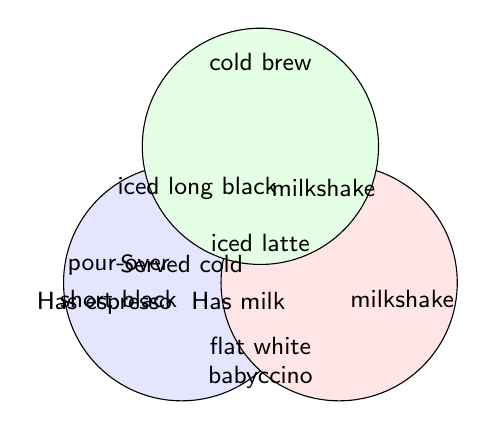
\begin{tikzpicture}[font=\sffamily, every node/.style={font=\sffamily\small}]
  % Define circle centers
  \coordinate (A) at (0,0);   % Has espresso
  \coordinate (B) at (2,0);    % Has milk
  \coordinate (C) at (1,1.732); % Served cold

  % Draw circles with labels
  \draw[fill=blue!10] (A) circle (1.5cm) node[pos=0.5, below left] {Has espresso};
  \draw[fill=red!10] (B) circle (1.5cm) node[pos=0.5, below right] {Has milk};
  \draw[fill=green!10] (C) circle (1.5cm) node[pos=0.5, above] {Served cold};

  % Place drinks in correct regions
  % Espresso only (left, not overlapping)
  \node at (-0.8, -0.2) {short black};
  \node at (-0.8, 0.2) {pour-over};
  
  % Milk only (right, not overlapping)
  \node at (2.8, -0.2) {milkshake};
  
  % Cold only (top, not overlapping)
  \node at (1, 2.8) {cold brew};
  
  % Espresso ∩ Milk (bottom overlap)
  \node at (1, -0.8) {flat white};
  \node at (1, -1.2) {babyccino};
  
  % Espresso ∩ Cold (left-top overlap)
  \node at (0.2, 1.2) {iced long black};
  
  % Milk ∩ Cold (right-top overlap)
  \node at (1.8, 1.2) {milkshake};
  
  % All three (center)
  \node at (1, 0.5) {iced latte};

\end{tikzpicture}
\end{document}
